%% Submissions for peer-review must enable line-numbering
%% using the lineno option in the \documentclass command.
%%
%% Preprints and camera-ready submissions do not need
%% line numbers, and should have this option removed.
%%
%% Please note that the line numbering option requires
%% version 1.1 or newer of the wlpeerj.cls file, and
%% the corresponding author info requires v1.2

% \documentclass[fleqn,10pt, lineno]{wlpeerj} % for journal submissions
\documentclass[fleqn,10pt]{wlpeerj} % for preprint submissions
%\usepackage[nomarkers,figuresonly]{endfloat} % for placing the figures at the end of the document
\usepackage{textcomp} %for \textgreater
\usepackage{wasysym} %for \times
\usepackage{hyperref}

\title{Patterned progression of gut microbiota associated with necrotizing enterocolitis and late onset sepsis in preterm infants: a prospective study among a Chinese NICU}

\author[1]{Jiayi Liu}
\author[2]{Jianhua Sun}
\author[3]{Yuqing Li}
\author[4]{Yi Feng}
\author[5]{Liya Pan}
\author[6]{Zhoulonglong Xie}
\author[7]{Zhilong Yan}
\author[8]{Jianhua Zhao}
\author[9]{Li Hong}


\affil[1]{Department of Clinical Nutrition, Shanghai Children's Medical Center, School of Medicine Shanghai Jiao Tong University, Shanghai, China}
\affil[2]{Department of Clinical Nutrition, Shanghai Children's Medical Center, School of Medicine Shanghai Jiao Tong University, Shanghai, China}
\affil[3]{Department of Clinical Nutrition, Shanghai Children's Medical Center, School of Medicine Shanghai Jiao Tong University, Shanghai, China}
\affil[4]{Department of Clinical Nutrition, Shanghai Children's Medical Center, School of Medicine Shanghai Jiao Tong University, Shanghai, China}
\affil[5]{Department of Clinical Nutrition, Shanghai Children's Medical Center, School of Medicine Shanghai Jiao Tong University, Shanghai, China}
\affil[6]{Department of Clinical Nutrition, Shanghai Children's Medical Center, School of Medicine Shanghai Jiao Tong University, Shanghai, China}
\affil[7]{Department of Clinical Nutrition, Shanghai Children's Medical Center, School of Medicine Shanghai Jiao Tong University, Shanghai, China}
\affil[8]{Shanghai Majorbio Bio-Pharm Technology Co., Ltd, Shanghai, China}
\affil[9]{Department of Clinical Nutrition, Shanghai Children's Medical Center, School of Medicine Shanghai Jiao Tong University, Shanghai, China}
\corrauthor[9]{Li Hong}{hongli@scmc.com.cn}

%\keywords{Gut Microbiota, Preterm Infant, Necrotizing Enterocolitis, Neonatal Late Onset Sepsis, High Throughput DNA Sequencing}

%%%%%%%%%%   abstract  %%%%%%%%%%
\begin{abstract}
  Necrotizing enterocolitis (NEC) and late-onset sepsis(LOS) are two common complications of preterm infants with high morbidity and mortality. Recent studies in Europe and America had implicated dysbiosis of gut microbiota as a major contributing factor. Similar studies in Asian population remain scant. In this pilot study, we profiled gut microbiota of four NEC and three LOS patients among 24 preterm Chinese infants starting from birth till decease or discharge.  The microbial community diversities in case samples differed significantly from those of controls. These differences emerged after the third day of life and persisted throughout the courses of both NEC and LOS. Similar to previous studies, the microbiota of cases are less diversified.  However, using  Zero-Inflated Beta Regression Model with Random Effects (ZIBR) we observed  higher \textit{Bacillus} (p = 0.032) and \textit{Solibacillus} (p = 0.047) in the onset  both NEC and LOS patients. Moreover, these changes in diversity and composition preceded the onset of diseases and might have played an essential role in disease progression. During NEC progression, \textit{Enterococcus}, \textit{Streptococcus} and \textit{Peptoclostridium} were the dominant genera while \textit{Klebsiella} was the single dominant genus during LOS progression.  previous studies  These results warrant further studies to identify correspondent microbial patterns, etiological strains and underlying mechanisms
\end{abstract}

\begin{document}

\flushbottom
\maketitle
\thispagestyle{empty}

%%%%%%%%%%%%%%%%%%%%%%%%% INTRODUCTION %%%%%%%%%%%%%%%%%%%%%%%%%%%
\section*{Introduction}
The gut microbiota is a key contributor to human health. Imbalance of the microbial community, termed dysbiosis, is associated with various diseases, such as obesity and diabetes\citep{bouter2017role, rosenbaum2015gut,winer2016intestinal, cani2019severe, zmora2019}, immunity related diseases\citep{vogelzang2018microbiota, pronovost2019perinatal, Vatanen2016Variation}, neurodevelopmental disorders\citep{Sampson2015Control, pronovost2019perinatal}, cardiovascular diseases\citep{tang2017gut,Jie2017The, Jonsson2017Role} and cancers\citep{Gagliani2014The, Irraz2014The, Sears2014Microbes}.

The microbiota in newborn infants undergoes dynamic changes in composition, abundance and diversity before reaching a homeostasis status at around three years old\citep{yatsunenko2012human, backhed2015dynamics, stewart2018temporal}. Temporal colonization pattern of the intestinal microbiota during early stages of life may have important contribution to the long term health of individuals. Early life microbiota disruption had been associated with the development of metabolic and immunological  diseases such as Type I diabetes\citep{giongo2011toward, vatanen2018human}, asthma\citep{stokholm2018maturation} and allergy\citep{madan2012normal,savage2018prospective}.

In preterm infants, common medical practices including cesarean sections, formula feeding, sterile incubator nursing and extensive use of broad-spectrum antibiotics may limit normal micrbiota acquisition and development\citep{la2014patterned, shin2015first, Deweerdt2018How}. The abnormal colonization of gut microbiota may subject preterm infants to complications such as necrotizing enterocolitis (NEC) and late onset sepsis (LOS)\citep{Sharon2015Gut, Cernada2016Sepsis}.

Necrotizing enterocolitis is characterized by rapid ischemic necrosis of intestinal mucosa, resulting in high morbidity (2\% - 7\%) and mortality (15\% -30\%)\citep{neu2011necrotizing, stoll2015trends}. Its etiologies remain largely unknown and likely to be multifactorial. Previous studies in European and American countries have ssociated microbial dysbiosis to NEC onset. Reduction in microbiota diversity and unusual species colonization were observed in NEC patients\citep{jacquot2011dynamics,Warner2016a}. No causative species have been identified so far. However, increase in Proteobacteria phyla and decrease in Firmicutes was observed before NEC onset\citep{mai2011fecal, zhou2015longitudinal}. In addition, blooming of \textit{Gammaproteobacteria} and under-representation of \textit{Negativicutes} was associated with disease progression\citep{Warner2016a}.

Late onset sepsis (LOS) is another common life threatening disease of preterm infants. It is commonly defined as systemic infection with isolation of a bacterial pathogen from the bloodstream after 72 hours of life\citep{rao2016one, pickering2012red}. Preterm infants have immature gastrointestinal and immune system. Therefore, it is easier for  pathogenic bacteria or bacterial toxins to enter the bloodstream that may cause systemic inflammation\citep{schwiertz2003development, bezirtzoglou2011microbiota, Cernada2016Sepsis, Sharon2015Gut, korpela2018intestinal}, thus making the intestine a potential source of infections and inflammation. Previous studies showed that the LOS patients' gut microbiota was less diversified, and dominated by \textit{Staphylococci} and \textit{Enterobacter} but underrepresented by probiotic \textit{Bifidobacteria}\citep{madan2012gut,tarr2016gut,Stewart2017Longitudinal,korpela2018intestinal,ficara2018changes}.

China has a high rate of preterm birth rate at 7.1\%\citep{blencowe2012national}. Continuous improvements in neonatal health care has greatly improved survival of preterm infants in China.  However, it also increases the risk of developing NEC and LOS. Thus, elucidating their pathogenesis and developing preventive strategies would  greatly benefit  the health of preterm infants. Hence, we carried out a longitudinal pilot study to profile the microbiota of Chinese preterm NEC and LOS patients, with the aim to examine if similar alternations of microbiota correlate with disease onset and progression among Chinese patients. In line with previous studies in western countries, we observed lower bacterial diversity but higher variability among Chinese NEC and LOS patients.  However, we found that Chinese patients showed different bacterial compositions compared to western patients.


%%%%%%%%%%%%%%%%%%%%%%%%% METHODS %%%%%%%%%%%%%%%%%%%%%%%%%%%
\section*{Methods}
  \subsection*{Ethics}
  This study was approved by the joint committee of ethics of Shanghai Children’s Medical Center, Shanghai Jiao Tong University School of Medicine (SCMCIRB-K2013022). Detailed written informed consent was obtained from parents before enrolment.

  \subsection*{Patients}
  Newly born preterm infants with gestational age less than 33 weeks and birth weight over 950g were enrolled from Neonatal Intensive Care Unit at Shanghai Children’s Medical Center from July 2013 to December 2014. The exclusion criteria were 1) diagnosed with early-onset sepsis, 2) hepatic diseases, 3) renal impairment (Cr \textgreater 88 $\mu$M), 4) diagnosed with intestinal obstruction, 5) in foreseeable need of cardiovascular or abdominal surgeries (except for male circumcision or PDA ligation), 6) estimated parenteral support to supply over 50\% of daily caloric intake for more than four days, 7) given intravenous antibiotics administration (except prophylactic regimen of cefotaxime, piperacillin-tazobactam and/or metronidazole), 8) history of oral antibiotics administration, 9) grossly bloody stools at admission, and 10) over five days old.

  NEC cases were defined as infants who met the criteria for Stage II and Stage III NEC diagnosis\citep{bell1978neonatal}, including radiographic intestinal dilation, ileus, pneumatosis intestinalis, and/or absent bowel sounds with or without abdominal tenderness, and/or mild metabolic acidosis and thrombocytopenia. LOS cases was diagnosed if 1)an infant had a positive hemoculture or other suspicious loci of infection after 72 hours of life, with septic signs/symptoms reviewed independently by at least two neonatologists, and had been treated with advanced antibiotics (e.g., Meropenem) after diagnosis. Infants with no infectious complications were regarded as controls.

  \subsection*{Sample collection and handling}
  Fecal samples collection from neonatal meconium till decease or discharge, whichever comes first. Although we intended to collect fecal samples on a daily basis, due to working shifts and flexible clinical scheduling, we set seven days as the maximum interval between two collections from every infant. Every sample was collected from infants’ diaper with a sterile spatula into cryogenic vials within 30 minutes of defecation. The samples were immediately placed on dry ice and stored at - 80\textdegree{}C within 30 minutes without additives. All samples were collected and stored before knowing the diagnosis of respective patients.

  \subsection*{DNA extraction and quality control amplification and 16s rRNA gene sequencing}
  Microbial genomic DNA was isolated from each fecal specimen using the E.Z.N.A.® Soil DNA Kit (Omega Bio-Tek, Norcross, GA, U.S.) according to manufacturer’s protocols. The concentration and purity of the DNA were determined by NanoDrop 2000 UV-vis spectrophotometer (Thermo Scientific, Wilmington, USA), and the DNA quality was checked by 1\% agarose gel electrophoresis.

  \subsection*{Broad-range PCR and High-throughput Sequencing of 16s rRNA gene amplicons}
  The V3-V4 hypervariable regions of the bacterial 16S rRNA gene were amplified by PCR from each sample using bacterial\/archaeal primers 338F (5’-ACTCCTACGGGAGGCAGCAG-3’) and 806R (5’-GGACTACHVGG GTWTCTAAT-3’) using thermocycler PCR system (GeneAmp 9700, ABI, USA). The PCR reactions were as follows: 3 min of denaturation at 95 °C, 27 cycles of 30 s at 95 °C, 30 s annealing at 55 °C and 45 s elongation at 72 °C, and a final extension at 72 °C for 10 min. The PCR reactions were performed in triplicate, with each 20 $\mu$L mixture containing 4 $\mu$L 5X FastPfu Buffer, 2 $\mu$L 2.5 mM dNTPs, 0.8 $\mu$L of each primer (5 $\mu$M), 0.4 $\mu$L FastPfu Polymerase (TransGen Biotech, Beijing, China) and 10 ng template DNA.  PCR products were separated from impurities and genomic DNA by running in 2\% agarose gels.  The PCR bands were further purified using the AxyPrep DNA Gel Extraction Kit (Axygen Biosciences, Union City, CA, USA), and quantified using QuantiFluor™-ST (Promega, USA) according to the manufacturer’s protocols.
  Equimolar amounts of purified amplicons were pooled and paired ende sequenced (2 x 300) on an Illumina MiSeq platform (Illumina, San Diego, USA) according to the standard protocols of Majorbio Bio-Pharm Technology Co. Ltd. (Shanghai, China). The reads were de-multiplexed using the Illumina software and separate FASTQ files were generated for each specimen and deposited to the Sequence Read Archive NCBI under the BioProject accession PRJNA470548. Another public archive repository is available at \href{https://figshare.com/articles/Untitled_Item192_samples_for_publishing_Longitudinal_gut_microbiota_patterns_in_preterm_infants_with_necrotizing_enterocolitis_or_late-onset_sepsis_an_observational_prospective_study_/7205102}{figshare doi: 10.6084/m9.figshare.7205102}

  \subsection*{Raw Data Processing}
  Raw data was processed according to the standard protocols provided by Majorbio Bio-Pharm Technology Co. Ltd. (Shanghai China) as previously described\citep{liu2018splenectomy, wang2018bacterial}. In short, the protocols are as the followings:
  raw sequencing data was de-multiplexed. Sequence reads were subjected to quality filtering utilizing Trimmomatic software\citep{bolger2014trimmomatic} and were truncated at any site with an Phred score \textless 20 over a 50bp-sized window. Barcode matching with the primer mismatch from 0 to 2 nucleotides was adopted and reads containing ambiguous characters were removed. After trimming, FLASh(Fast Length Adjustment of Short Read)\citep{magovc2011flash}, a read pre-processing software, assembled and merged the paired-end reads from fragments and generated \textgreater 10 bp overlapped, with the dead match ratio 0.2. Unassembled reads were discarded. From the 192 fecal samples sequenced, a total of 7,472,400 optimized V3-V4 tags of 16s rRNA gene sequences were generated(Table S1).

  To unbiasedly compare all the samples at the same sequencing depth, the "sub.sample" command of mothur program(version1.30.1)\citep{schloss2009introducing} was used for normalization to the smallest sample size. Chimera was detected and removed by \href{https://www.drive5.com/usearch/manual/uchime_algo.html}{UCHIME Algorithm}. The effective reads were then sorted by cluster size and processed using Operational Taxonomic Units (OTUs) with 97\% similarity cutoff \href{http://drive5.com/uparse/}{UPARSE}-OTU algorithm (implementing "cluster\_otus" command)\citep{edgar2013uparse} in USEARCH(v10)(UPARSE version 7.1). The taxonomy of each 16S rRNA gene sequence was analyzed by \href{http://rdp.cme.msu.edu/}{RDP Classifier algorithm}\citep{wang2007naive} against the Silva (SSU128) 16S rRNA database\citep{quast2012silva} using confidence threshold of 70\%. Each sequence was assigned the taxonomy by QIIME\citep{caporaso2010qiime}. The representative sequences were allocated phylogenetically down to the domain, phylum, class, order, family, and genus levels. The relative abundance of a given taxonomic group was calculated as the percentage of assigned sequences over total sequences. From the 192 fecal samples sequenced, a total of 7,472,400 optimized V3-V4 tags of 16s rRNA gene sequences were generated.  We first analysed the chronological changes in microbiota richness among all three groups.

   Within-sample diversity(alpha diversity), including Shannon index and observed species richness (Sobs), were obtained using the "summary.single" command of mothur program(version1.30.1)\citep{schloss2009introducing}. Between-sample diversity(beta diversity) was obtained by calculating weighted UniFrac distances between samples.

  \subsection*{Statistical and Bioinformatics Analyses}
    \subsubsection*{Demographics and Clinical Sample comparisons}
    Kruskal-Wallis test and Wilcoxon rank-sum test were used to identify statistically significant differences in continuous variables, including gestational age, birth weight, age at diagnosis and length of hospitalization. The $\chi^2$, or Fisher's exact test were used to identify differences in gender composition. $\alpha$ level was considered 0.05 for all statistical tests. Other statistical tests not involving microbiome 16s rRNA sequencing data were performed using \textit{"stats"} package using R(v.3.5.1).
    \subsubsection*{Microbiota and Bioinformatics Analyses}
      \paragraph*{Disease-related Time Interval Definition}
      Considering that the sampling and disease onset timepoints for each patient were not perfectly universal, to illustrated the continuous longitudinal and repeated nature of the sampling and its relationship with onset and progression of diseases, we splitted the whole sampling span into 7 time intervals:
        \begin{enumerate}[noitemsep]
          \item early post-partum(EPP): within 3 days afterbirth
          \item early pre-onset(EPO): from the end of EPP to at least four days before disease onset
          \item late pre-onset(LPO): from the end of EPO to the start of onset; for control group patients, the equivalent onset time is set at 16 days of life, as is the average diagnosis age of NEC and LOS groups.
          \item early disease(ED): first third interval of whole disease span; for the control group, for the control group, the equivalent ED interval is from the day 16  to discharge.
          %\item early disease equivalent(EDe): from the 16th day of life until discharge for control group. This time interval is exclusively set for the control group, which is equivalent to the ED interval in NEC and LOS groups.
          \item middle disease(MD): second third interval of whole disease span
          \item late disease(LD): last third interval of whole disease span
          \item post disease(PD): from the end of disease to discharge time-point
        \end{enumerate}

      \paragraph{Diversity Analyses}
      The average of $\alpha$  diversity of each patient was calculated, if more than two samples were available within one analysis interval. Kruskal Wallis tests were used to compare the alpha diversity differences.   Differences in time-with-disease alpha diversity were analyzed by a two-way repeated measures ANOVA, with time interval (EPP, EPO, LPO, ED, MD, LD, PD) as a within-subject factor and group (NEC, LOS, control) as a between-subject factor.

      \paragraph*{Modeling Strategies for Taxonomy Comparisons}
      To compare the dynamics of microbiota diversity and relative taxonomic abundance preceding the disease, we took the EPP, EPO, LPO and ED interval among all patients into the ZIBR model (supplementary matrix1).
      To compare the microbiome profile right after birth until disease alleviation, we selected EPP, EPO, LPO, ED, MD and LD interval of NEC and LOS patients(Supplementary matrix2 dataset) and fit the data into the model.
      The average taxonomy relative abundances, if more than two were available within one analysis interval, of each patient was calculated.
      Zero-Inflated Beta Regression Model with Random Effects (ZIBR) and Linear Mixed-effects Model(LME) were used to test the association between OTU relative abundance and clinical covariates (diseases-related time intervals) for longitudinal microbiome data \citep{chen2016two}. \textit{ZIBR} and \textit{nlme}\citep{nlme} R packages were utilized for each model.

    \subsubsection*{Scripts and Figures Archiving}
    Figures were generated with the \textit{"ggpubr"}\citep{kassambara2017ggpubr},  \textit{"ggplot2"}\citep{ggplot2} and \textit{"ggsci"}\citep{ggsci} packages using R(v.3.5.1).
    Scripts for modeling and figures plotting, input and output files, figures are available at our \href{https://github.com/jiayiliujiayi/NEC-LOS-microbiota_pattern_comparison}{github repository}.



\section*{Results}
  \subsection*{Patients characteristics}
   From July 2013 to December 2014, a total of 130 preterm infants admitted to the neonatal intensive care unit (NICU) of Shanghai Children’s Medical Center met the criteria of our study and a total of 1698 samples were collected.  We sequenced 192 fecal samples from 24 well-sampled preterm infants.  Four were subsequently diagnosed with NEC (2 in stage IIA and 2 in stage IIB) and three with LOS (2 with positive hemoculture of Klebsiella pneumoniae; the other 1 was diagnosed upon sepsis-related signs and symptoms, lab test of white blood cells \textgreater 20 cells/microL and her effective reaction to vancomycin).  The remaining 17 were used as matched controls (Figure\ref{fig:design}, Supplemantary Table S2). Fecal samples were collected between days 1 and 69 of life. Numbers of samples collected and interval of sampling varied among patients but met our preset criteria of less than 7 days between sampling. The average number of sample collected for NEC, LOS and normal control patients was 15, 10 and 6 respectively.  Number of sample per patients was higher for the NEC and LOS group than the control group because of longer period of hospitalization.
     \begin{figure}[!htbp]\centering
       \includegraphics[width=\linewidth]{figure/patinfo.pdf}
       \caption{Schematic of Study Design}
       \label{fig:design}
     \end{figure}

     \emph{Fig 1. Schematic of Study Design. Longitudinal fecal samples were collected over from birth to decease or discharge from preterm infants in the NICU. Bacterial diversity and compositions were then characterized. Image credit: Icons made by Freepik from \href{www.flaticon.com}{www.flaticon.com}}

   All 24 infants sampled were delivered by cesarean section, fed on infant formula and prescribed with prophylactic antibiotics regimen of cefotaxime, piperacillin-tazobactam and/or metronidazole right after they were admitted to our NICU. No infant was prescribed probiotics during hospitalization. There was no significant difference in gestational age (p = 0.074), birth weight (p = 0.11) or gender proportions (p = 0.820) among three groups. The average age at diagnosis for both disease group was 16 days and there was no statistical difference between the groups (p = 0.629) (Table~\ref{tab:demographic}). Therefore, we assigned day 16 until discharge as early disease interval, day 4-8 as early pre-onset interval, day 9-15 as late pre-onset interval for the control group.
    \begin{table}[!hpb]
       \centering
       \caption{\label{tab:demographic}Demographic characteristics of Preterm NEC, LOS and control groups.}
      \begin{tabular}{lp{1.8cm}p{1.8cm}p{1.8cm}p{2cm}c}
        \toprule
          & \textbf{NEC (N=3)} & \textbf{LOS (N=4)} & \textbf{Control (N=17)} & \textbf{Statistical Test} & \textit{p value} \\ \midrule
        \textbf{Gestational Age (weeks)} & 29(29-30) & 30(29-31) & 31(28-33) & Kruskal-Wallis test & 0.074 \\
        \textbf{Birth Weight(g)} & 1416.3 (773.4-2149.1) & 1141.7 (633.4-1649.9) & 1527.4 (1391.6-1663.1) & Kruskal-Wallis test & 0.111 \\
        \textbf{Gender} &  &  &  & Fisher's exact test & 0.820 \\
        \multicolumn{1}{r}{Female} & 3(75\%) & 2(67\%) & 9(53\%) &  & \\
        \multicolumn{1}{r}{male} & 1(25\%) & 1(33\%) & 8(47\%) &  & \\
        \textbf{Diagnosis Age(days)} & 16(11-19) & 16(10-22) & — & Wilcoxon rank-sum test & 0.629 \\
        \textbf{Length of Stay(d)} & 54.3 (13.5-95.0) & 60.0 (24.8-95.2) & 32.9 (26.3-39.5) & Kruskal-Wallis test & 0.046 \\
        \textbf{Number of Samples} & 46 & 42 & 103 & — & — \\ \bottomrule
      \end{tabular}
    \end{table}

   \subsection*{Longitudinal Microbiome Diversity of NEC and LOS patients}
    To get an overview of gut microbiota in patients, we analysed the gut microbiome richness of the NEC and LOS patients over time.  Similar to the normal group, the case groups showed similar microbiota richness trend from early post-partum (EPP) to early disease (ED), with the observed species (Sobs) decreased significantly from early post-partum stage (EPP) to early disease (ED) stage (Fig\ref{fig:sobs-group-time} a. control group, p \textless 0.01; b. NEC group, p = 0.044; c. LOS group, p = 0.013; ; supplemantary!!! rm-matrix1-sobs, two way RM ANOVA, p \textless 0.0001).  The biggest decrease in richness was between early pre-onset (EPO) to late pre-onset (LPO).  However, the decrease in the disease groups was less significant than the control group (NEC group p = 0.18, LOS group p = 0.066, normal p = 0.0004). The Sobs then stabilized from LPO onward with no significant difference between adjacent time intervals.

    \begin{figure}[ht]\centering
      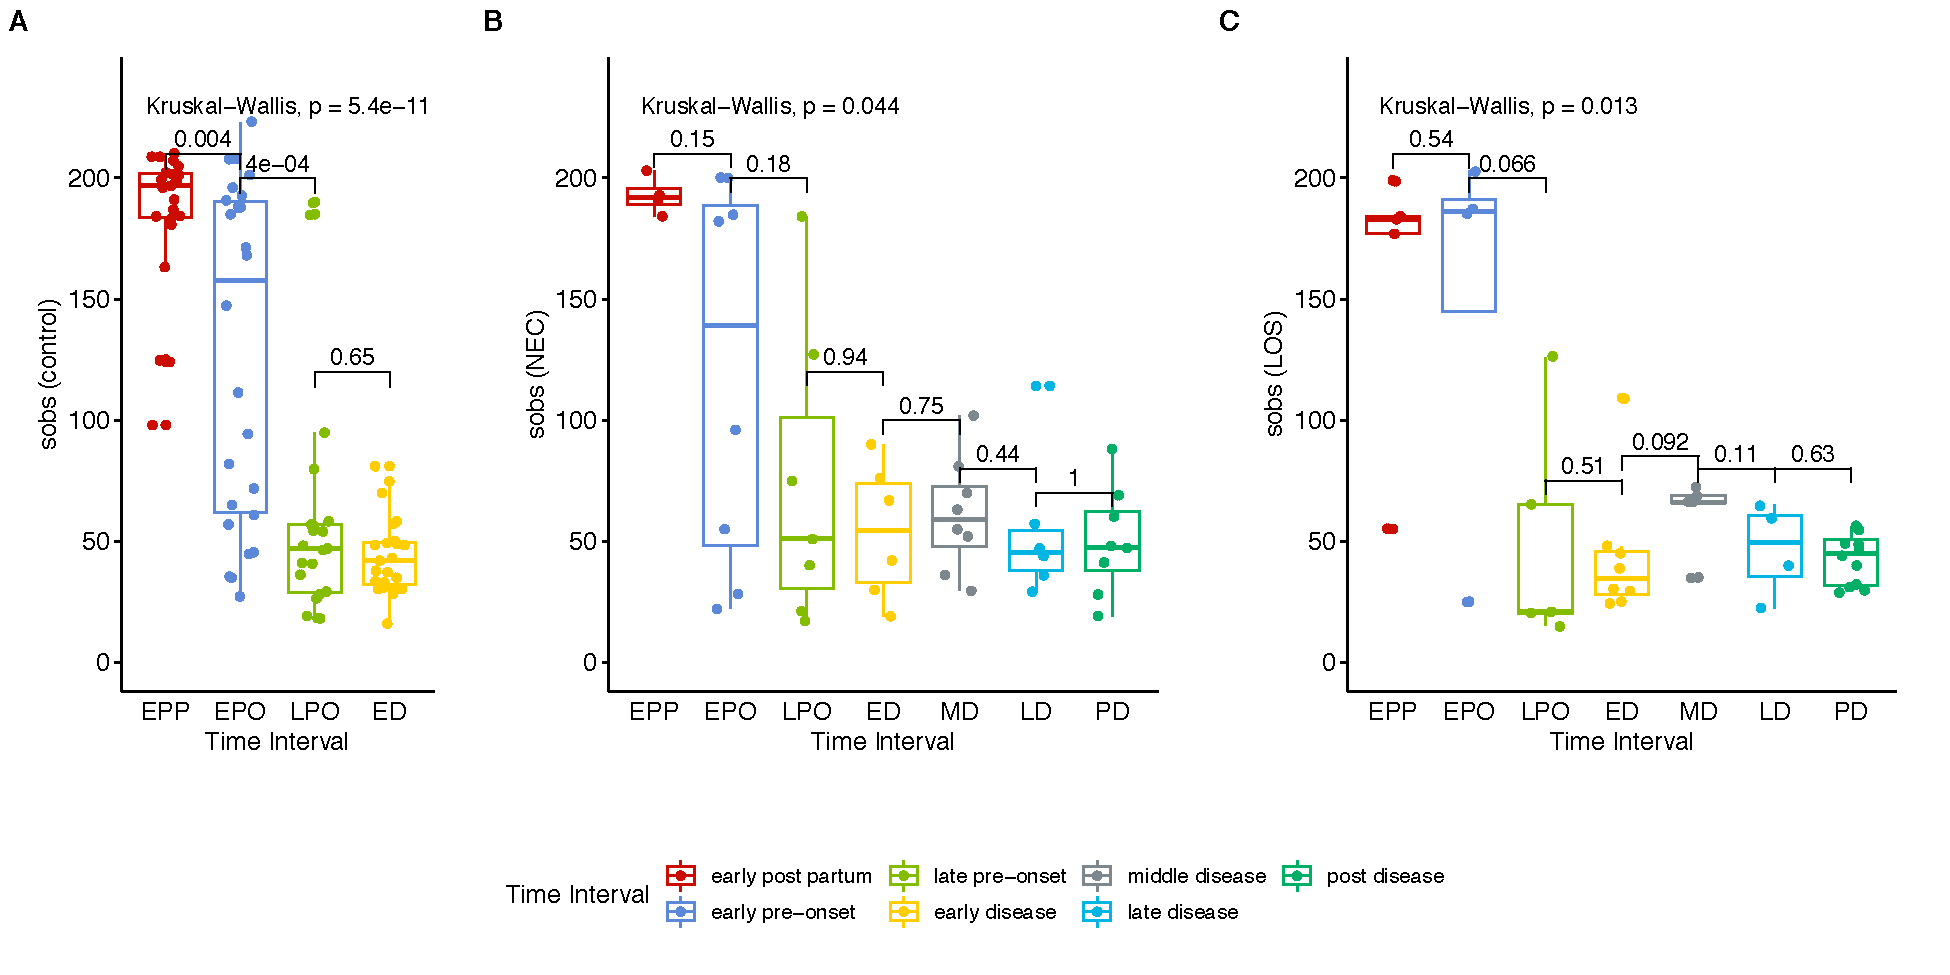
\includegraphics[width=\linewidth]{figure/sobs-group-time2.pdf}
      \caption{Trend in microbiome richness (Sobs) over time.}
      \label{fig:sobs-group-time}
    \end{figure}

    \textit{Fig2 Trend in microbiome richness (Sobs) over time. \\ Microbial richness trend in case and controls (a. NEC group, b. LOS group, c. control group). Horizontal line shows median, box boundaries show 25th and 75th percentiles. Sobs index value of each sample is depicted as one dot. }

    Next, we analyzed gut microbiome evenness represented. Similar to microbiota richness,  the shannon indices decreased from early post-partum (EPP) to early disease (ED) stages (Fig\ref{fig:sobs-group-time}). The shannon index of the control group decreased significantly (p = 0.04 from early postpartum (2.768) to early disease (1.004)).  Similarly, the shannon index of the NEC group also decreased significantly (p = 0.01) from early post-partum (3.141) to early disease stage (0.578) while that of LOS group decreased from (2.641) to (0.470) (p = 0.01)

    \begin{figure}[ht]\centering
      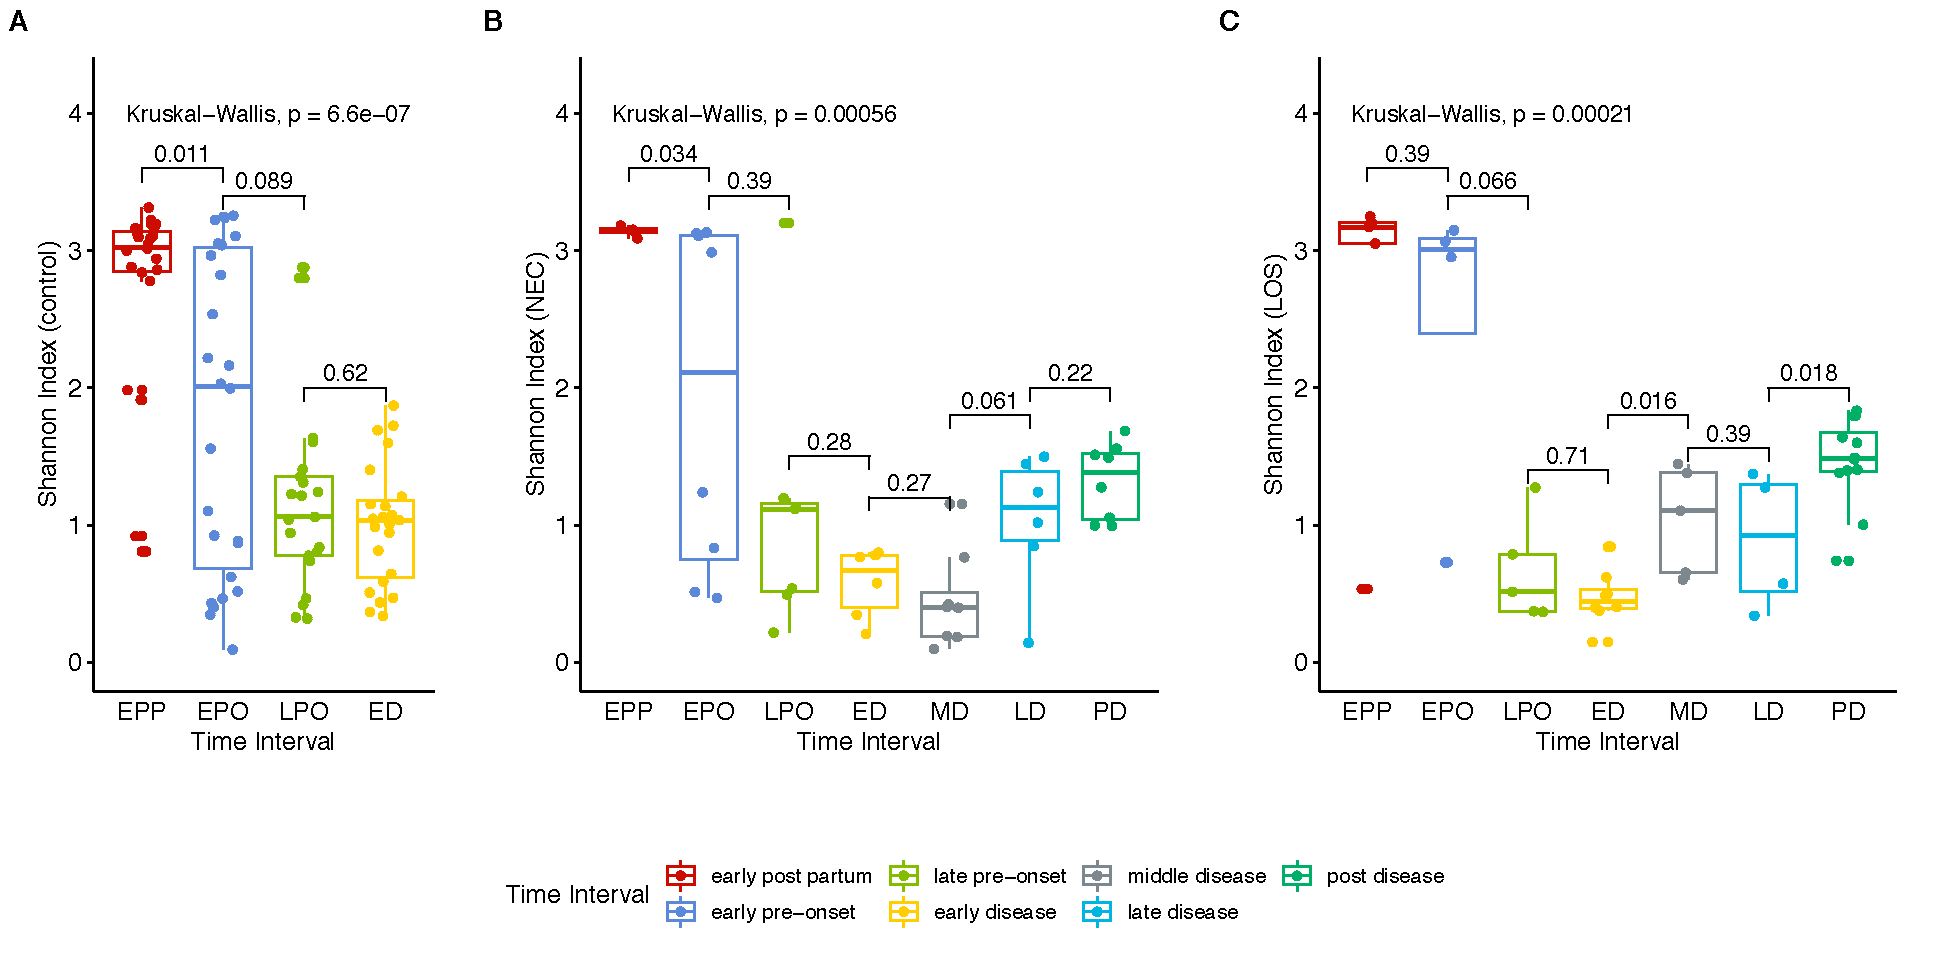
\includegraphics[width=\linewidth]{figure/shannon-group-time2.pdf}
      \caption{Post-partum microbiome evenness (Shannon) trend in each group.}
      \label{fig:shannon-group-time}
    \end{figure}

    \textit{Fig3. Post-partum microbiome evenness (Shannon) trend in each group. \\ Shows microbial richness trend in stools from cases and controls (a. NEC group, b. LOS group, c. control group). Horizontal line shows median, box boundaries show 25th and 75th percentiles.  Shannon index value of each stool is depicted as one dot. p=0·004 for NEC and p = 0.010 for LOS from early pre-onset to early disease indicating significantly discordant trends in bacterial diversity preceding disease onset. }

    Two way RM ANOVA showed significant shannon index divergent among three groups before disease onset (EPP to ED, p = 0.0017, supplemeantary matrix1). Moreover, during early disease stage, the shannon indices were different among three groups (Fig\ref{fig:shannon-time-groups}, facet ”early disease”, p = 0.0037), suggesting that microbiota distortion may precede NEC and LOS onset. As diseases progressed, the NEC group differed significantly with the the LOS group during middle disease interval but insignificantly  during late disease interval (Fig\ref{fig:shannon-time-groups} facet ”middle disease”, p = 0.034; facet ”late disease”, p = 0.750). Finally, alleviation of both diseases increased the shannon indices back to the early pre-onset levels (Fig. 3 b. NEC, early pre-onset at 1.925 vs. post disease at 1.320, p = 0.79; Fig3c. LOS, early pre-onset at 2.473 vs. post disease at 1.463, p = 0.16).

    \begin{figure}[ht]\centering
      \includegraphics[width=\linewidth]{figure/shannon-time-groups.pdf}
      \caption{Post-partum microbiome evenness (Shannon) in each time-interval. }
      \label{fig:shannon-time-groups}
    \end{figure}
    \textit{Fig4. Post-partum microbiome evenness (Shannon) in each time-interval. \\ Shows microbial richness trend in stools from cases and controls (a. NEC group, b. LOS group, c. control group). Horizontal line shows median, box boundaries show 25th and 75th percentiles.  Shannon index value of each stool is depicted as one dot. p=0·004 for NEC and p = 0.010 for LOS from early pre-onset to early disease indicating significantly discordant trends in bacterial diversity preceding disease onset. }

    \subsection*{Kinetics of Microbiome Composition}
    To compare the beta-diversity of the three groups over time, we applied Principal Component Analysis (PCoA) to weighted UniFrac distance matrix.
    During early post-partum interval, beta-diversity among three groups was the lowest with the first principal coordinates accounted for 33.01\%. Then beta diversity continued to drift away from one another. The first principal coordinate one (PC1) increased from 33.01\% at early post-partum to 35.23\% at early pre-onset stage, 38.36\% at late-onset stage and eventually reaching 42.32\% at early disease stage (Fig\ref{fig:pcoa} b to d).  This continuous increase in beta-diversity suggested that the phylogenetic composition of the patients’ microbiome started to deviate from the control group before the onset of diseases. As disease progress, the phylogenetic similarity between the NEC and the LOS disease groups separated further and peaked at 59.53\% at middle disease stage then came down gradually to 42.8\% at post disease stage (Fig\ref{fig:pcoa} e to g) This trend in phylogenetic dissimilarity suggested that the microbiome composition of the NEC and LOS patients might have deviated from normal even before the onset of diseases.  While the further separation between the NEC and the LOS groups could be a result of different treatment strategies.
    \begin{figure}[ht]\centering
      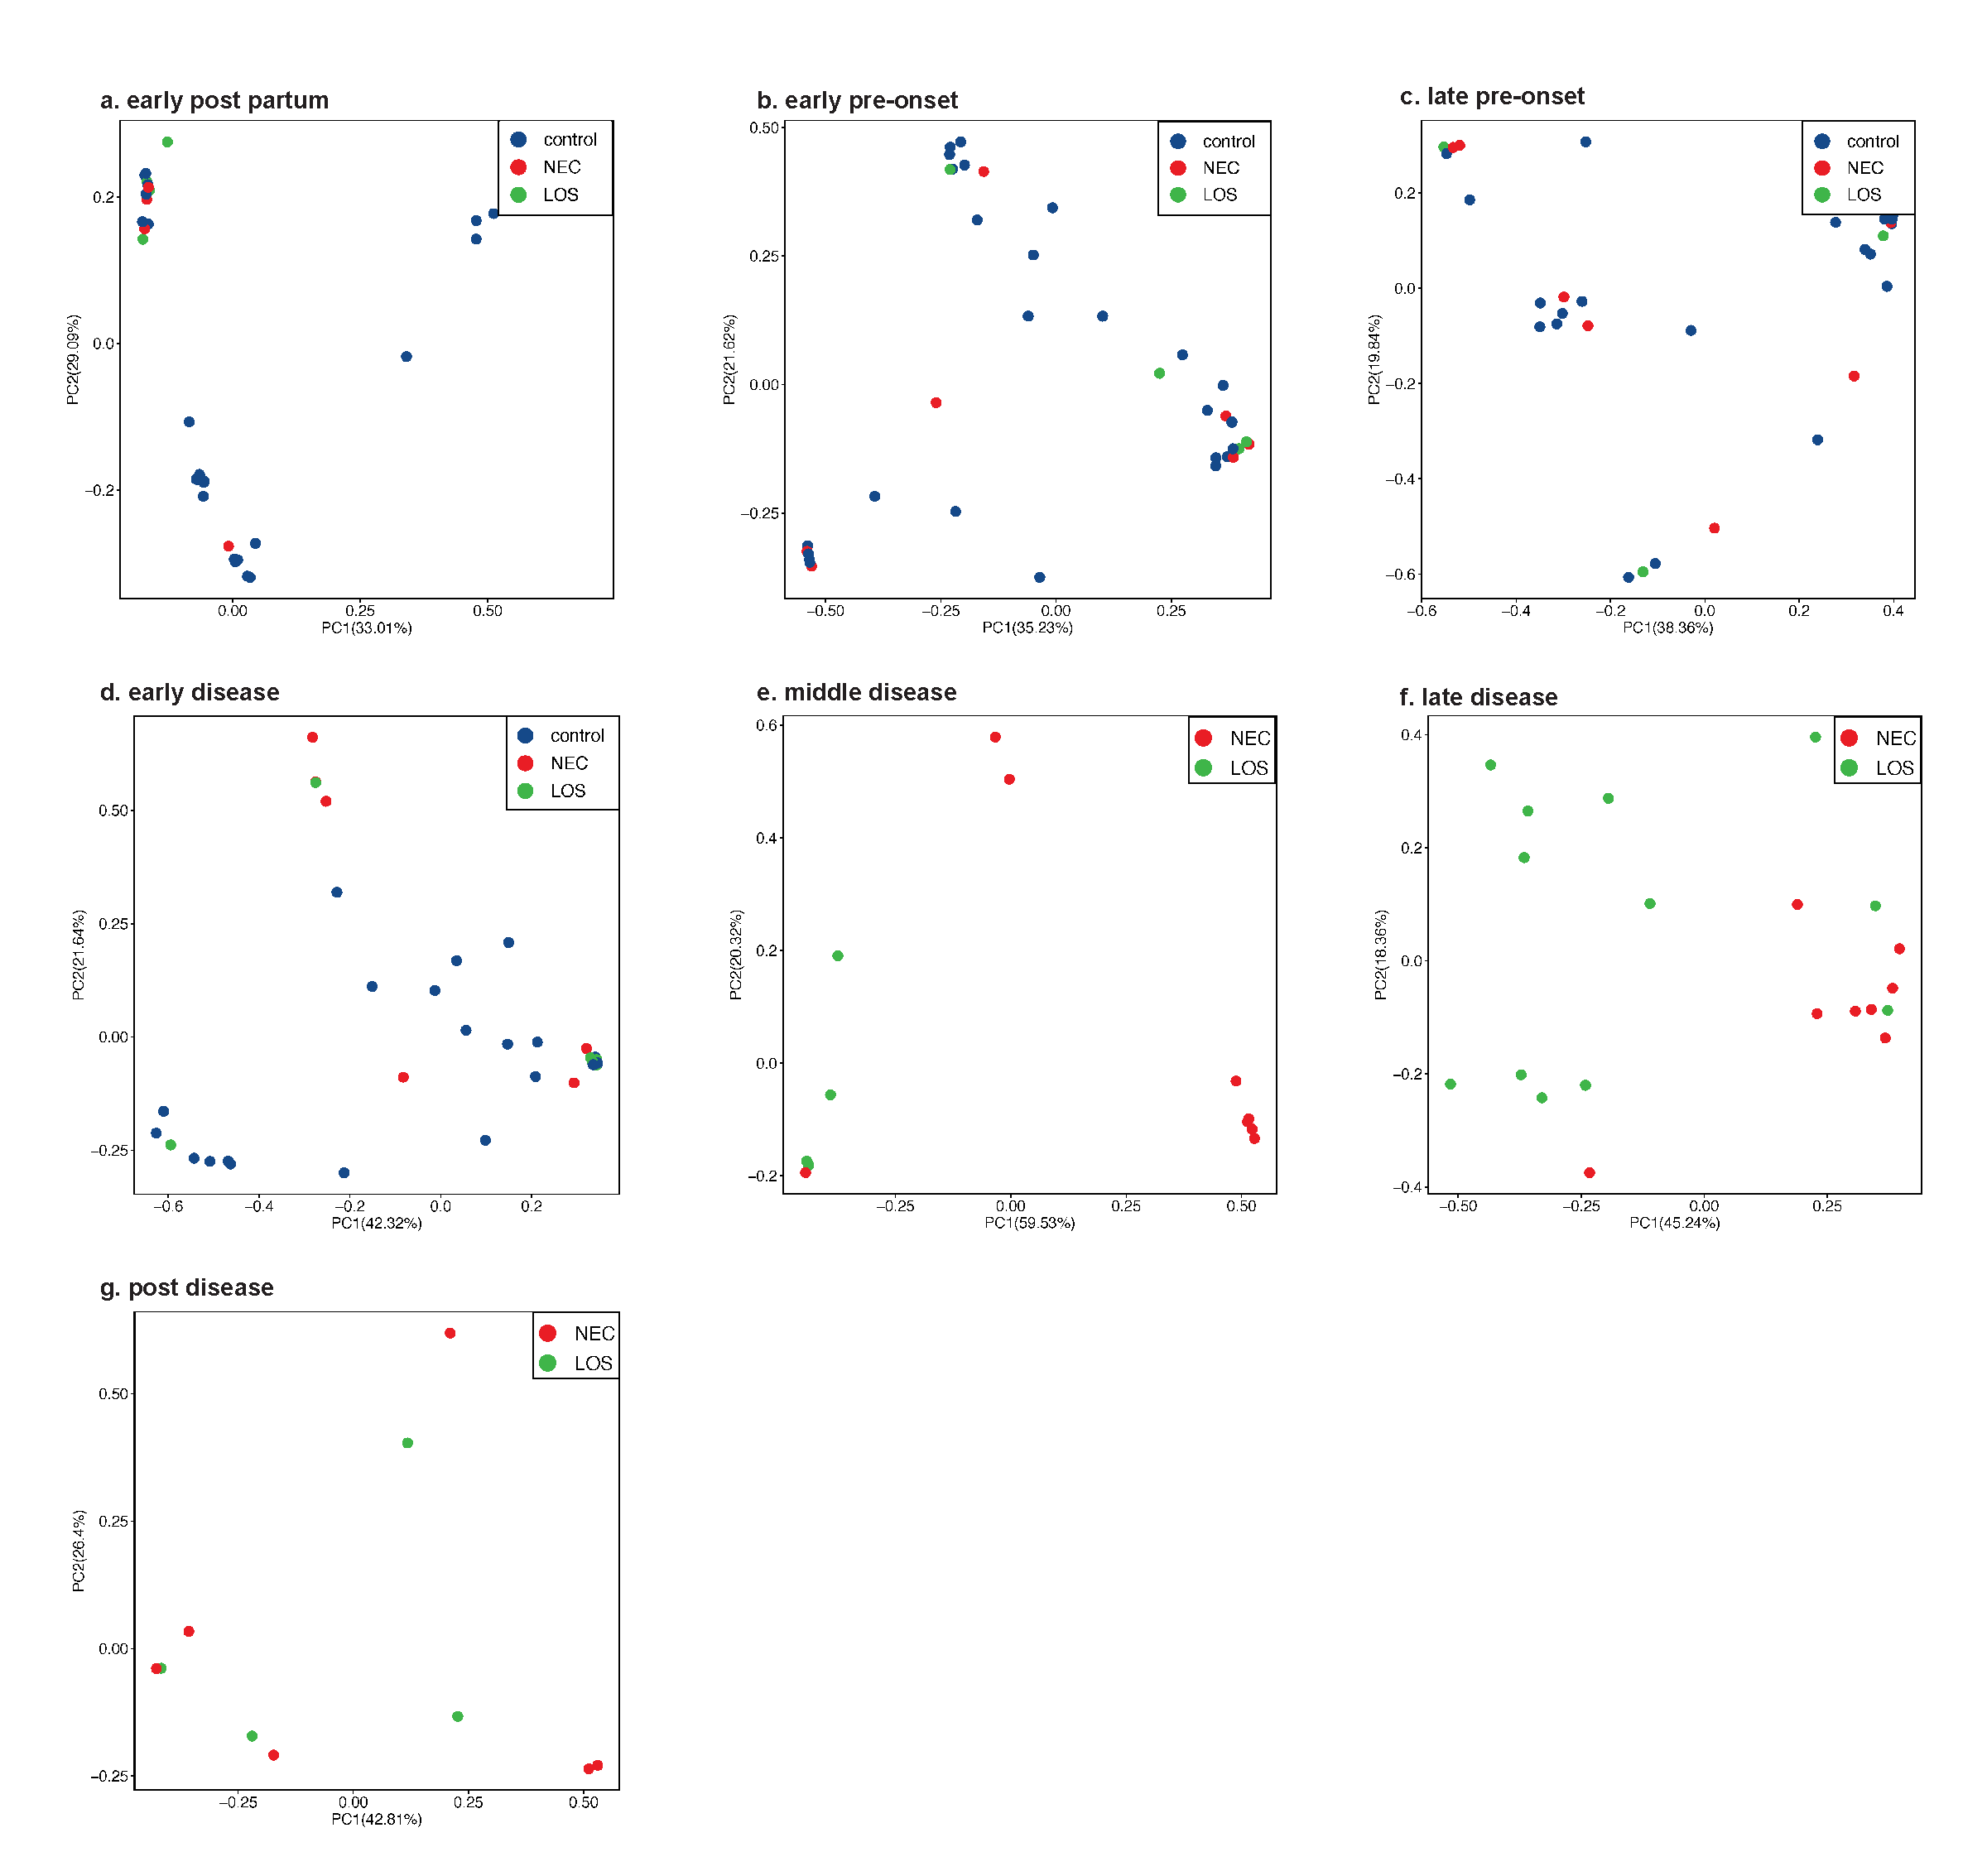
\includegraphics[width=\linewidth]{figure/pcoa_time_group.pdf}
      \caption{Beta diversity of the NEC, LOS and the control groups over time.}
      \label{fig:pcoa}
    \end{figure}


    \emph{Fig 5. Beta diversity of the NEC, LOS and the control groups over time. Beta diversity of samples is depicted by principal coordinates analysis ‘PCoA’ plot showing unweighted UniFrac distance between samples. Each dot represents the microbiota of a single sample.  Samples from the same group is represented by the same colors. Scatter plot shows principal coordinate 1 (PC1) versus principal coordinate 2 (PC2). Percentages shown are percentages of variation explained by the components. Samples that clustered closer together are considered to share a higher proportion of the phylogenetic tree and represented by a lower percentage in PC1.}

  \subsection*{Colonization Trend at Genus Level}
  In the analyses of microbiome alpha(Fig\ref{fig:sobs-group-time,}) and beta diversity(Fig\ref{fig:shannon-group-time, fig:shannon-time-groups}), detectable differences was observed among the three groups, especially during transition from LPO to ED stage.  This indicated that the microbiota assembly of the two disease groups and the normal group might be different.  To further investigate if any change in microbiota composition correlate with the onset and/or progression of NEC and LOS, we tracked the changes in bacteria at genus level during hospitalization.  We filtered the genus of over 10\% relative abundance among all samples and plotted relative abundance over time(Fig\ref{fig:taxa-time}).

  \begin{figure}[ht]\centering
    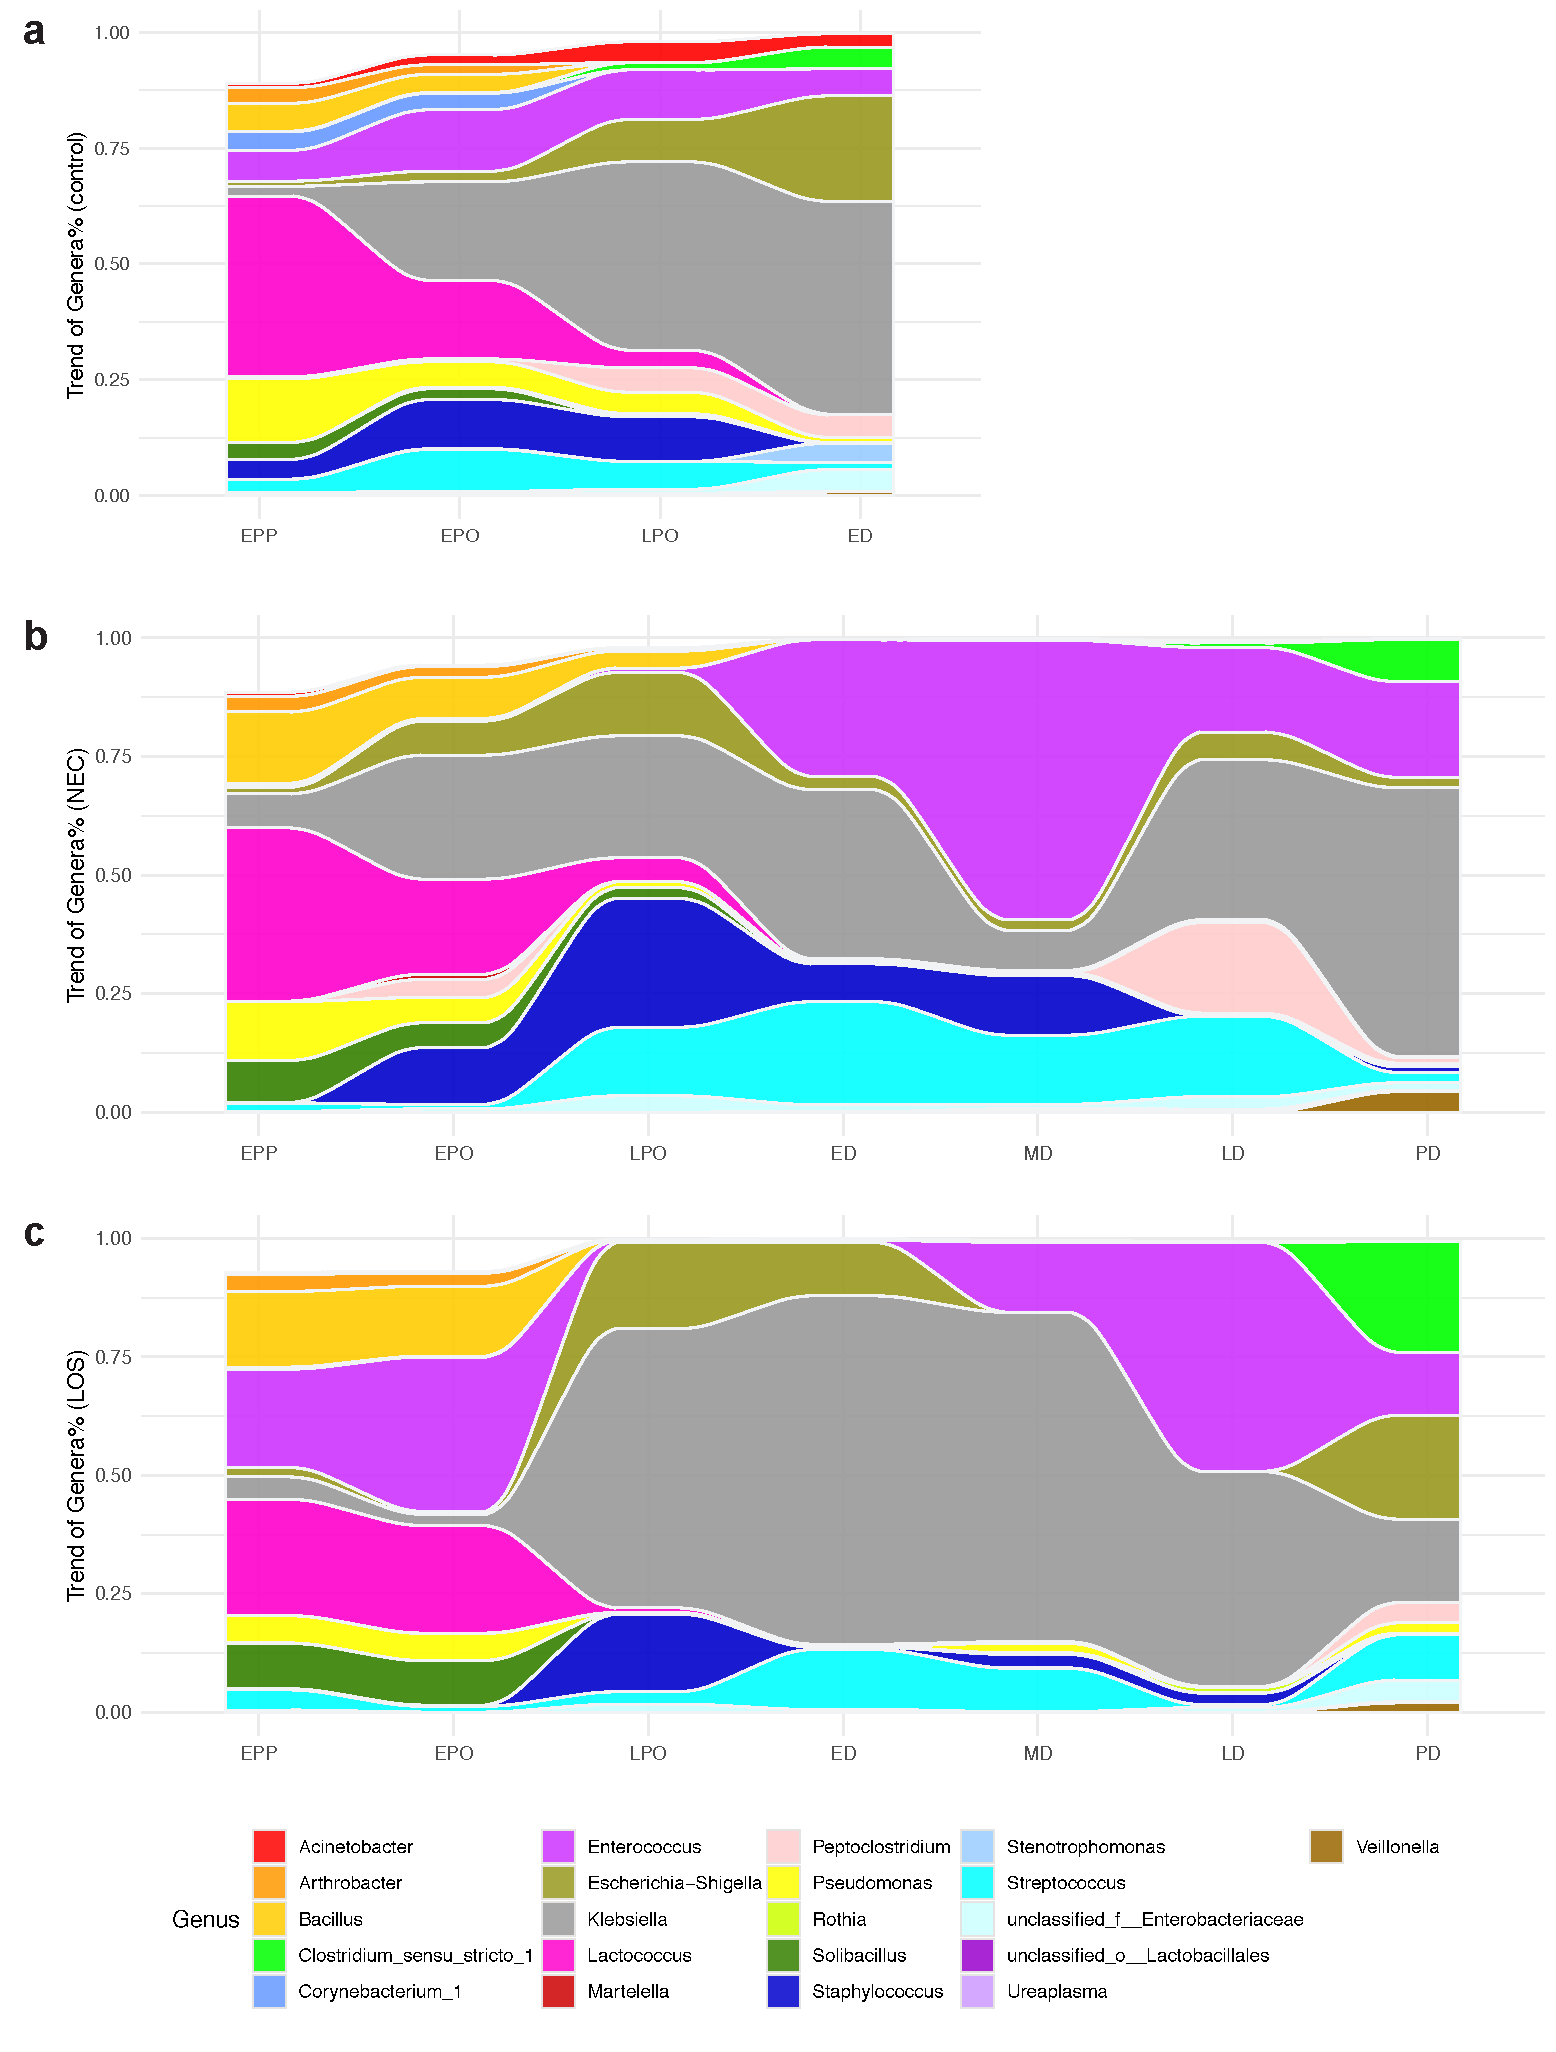
\includegraphics[width=\linewidth]{figure/taxon.pdf}
    \caption{Alluvial diagrams showing temporal development of microbiome in three groups}
    \label{fig:taxa-time}
  \end{figure}

    At early post-partum stage, all three groups showed high proportion of Lactococcus, Bacillus and Pseudomonas. However, ZIBR model the disease groups showed significantly higher OTUs that matched to Bacillus (NEC 15.05\% and LOS 15.97\% compare to 6.02\% of controlnormal, p = 0.032) and Solibacillus and higher Solibacillus (8.88\% in NEC and 9.61\% in LOS compare to 3.65\% of controlnormal, p = 0.047) from the case groups (ZIBR table cited). Moreover, Enterococcus proportion (Fig\ref{fig:taxa-time}a, purple area) was much higher in LOS patients (20.72\%) than the normal controls (6.66\%, Fig. 6a, purple area) but almost absent in NEC patients (0.51\%) (Fig\ref{fig:taxa-time}b).  While all three groups showed increases in Klebsiella and Escherichia-Shigella, and decreases in Lactococcus from EPP to ED, the rates of change were different among the three groups.  The LOS group exhibited the most drastic changes, with rapidly increased of Klebsiella (from 4.71\% to 58,90\%), Escherichia-Shigella (from 2.02\% to 18.16\%) and Streptococcus (from 1.22\% to 12.68\%).(Fig\ref{fig:taxa-time}c).  Together, these three genera accounted for almost  100\% of all bacteria (Fig 6c).  In addition, Lactococcus decreased more rapidly than the other groups, from 24.5416.0\% at EPP to 0.94002\% before LPO (Fig\ref{fig:taxa-time}c. magenta area).

  	On the other hand, increase of Klebsiella was the smallest  in NEC patients (Fig\ref{fig:taxa-time}b grey area, from 7.17\% at EPP to 35.63\% to ED).  Moreover, a rapid surge of Enterococcus, Staphylococcus and Streptococcus from EPO to ED was only observed in NEC patients (Fig. 6b, purple, dark and light blue area).

  	As disease progress with medical intervention, the composition of the disease group underwent another round of drastic changes.  Most notably, the fluctuation of Enterococcus, Klebsiella, Staphylococcus and Peptoclostridium during the disease stages (Fig\ref{fig:taxa-time}b and c, stage ED to LD).  This might be the result of difference regimen of antibiotics used to treat NEC versus LOS.  Interestingly, as patients approached remission, the composition became more balanced, more resembled that of the normal control, except a higher level of Clostridium.  In summary, compare to normal preterm infants, we observed different patterns of temporal changes in bacterial composition among NEC and LOS patients.  Rapid changes in relative abundance of certain genera were revealed as early as early pre-onset of stages.  These changes were especially obvious in LOS patience.

  \textit{Fig 6. Alluvial diagrams showing temporal development of microbiome in three groups. Genus of relative abundance over 10\% were depicted. a. control group, b. NEC group, c. LOS group}

%Bar graph depicting the relative abundance of most commonly encountered bacterial phyla between FT, ELBW and BPD infants.

%%%%%%%%%%%%%%%%%%%%%%%%%%%%%% DISCUSSION %%%%%%%%%%%%%%%%%%%%%%%%%%%%%
\section*{Discussion}
%NEC and LOS are major causes of morbidity and mortality in preterm infants worldwide and have been exerting economic burdens on healthcare costs\citep{johnson2013cost,johnson2014economic, mowitz2018cost}. Although early recognition and treatment regimen has improved clinical outcomes, both diseases still account for morbidites in NICU survivors\citep{hintz2005neurodevelopmental, zonnenberg2019neurodevelopmental, shah2015risk}. China has a high rate of preterm birth at 7.1\%\citep{blencowe2012national}. Continuous improvements in neonatal health care greatly improved survival of preterm infants in China.  However, it also increased the risk of developing NEC and LOS. Thus, elucidating their pathogenesis and developing preventive strategies would  greatly benefit  the health of preterm infants.

In this pilot study, we intended to investigate the etiopathology of NEC and LOS in Chinese preterm infants from a intestinal-microbial perspective. We profiled the gut microbiome of NEC and LOS patients from birth to decease/discharge. Every infant in our cohort was c-setion delivered, fed by infant formula and administered antibiotics starting from the first day of life. [The sample size was relatively small.  However, some of our findings is similar to that conducted in western countries. Should this be mentioned in the "limitation" part? ].  Mainly, infants who developed NEC or LOS exhibit a different gut microbiota colonization pattern relative to the controls. Case groups showed decline in diversity, although to different extent. Moreover, NEC and LOS infant' intestine were prone to harbor potential pathogens during both pre-onset and disease stage, such as \textit{Enterococcus}, \textit{Staphylococcus}, \textit{Peptoclostridium} and \textit{Streptococcus}.

To our knowledge, few studies has analyzed stool bacterial diversity in preterm infants as early as three days after birth. Strikingly, the bacterial richness and evenness among all three groups were the highest within three days after birth (i.e. early post-partum interval). However, a generally declining trend of microbial alpha diversity was observed afterwards in both case groups and the control group. The number of colonized species (sobs index) over time, in line with previous studies\citep{mai2011fecal, mai2013distortions}, remained similar before disease onset in all three groups (might be largely due to the similar nursing environment within the NICU from which the infants acquired mostly their gut microbiota?), suggesting the minor role of bacterial richness in the disease onset. Furthermore, the pervasive effect of antibiotics in reducing microbial richness has been reported in preterm infants: decrease in bacterial richness and diversity was reported 1 week to 2 months after early-life antibiotics\citep{digiulio2008microbial, dethlefsen2011incomplete, fouhy2012high, greenwood2014early, tanaka2009influence}. In our cohort, all the patients were administered with standardized antibiotic regimen right after hospitalization. The drastic decrease in sobs from early to late pre-onset interval (3 to 16 days of life), however, showed an earlier and more instant effect of antibiotics.

Furthermore, microbiota beta-diversity, which measures the phylogenetic similarity of stool microbiota (using a weighted UniFrac based PCO analysis), drifted away continuously after birth among three groups until alleviation of both disease. These findings were in accordance with a previous study showing that the microbiota of NEC patients were similar to that of the health controls\citep{mai2011fecal}; while inconsistent with previous findings that the microbiota within 72 hours before onset resembled that during disease stage in LOS patients\citep{mai2013distortions}.

Roles of empiric prophylactic antibiotics in NEC or LOS are controversial. In animal models, antibiotics eliminating Gram-negative bacteria enhance gut function and diminish mucosal injury to the bowel thus preventing necrotizing enterocolitis or bacterial leakage into the bloodstream\citep{carlisle2011gram, jensen2013antibiotics, birck2015enteral}. In clinical practices, broad-spectrum antibiotics (the most commonly prescribed medicine in the NICU) are recommended to empirically prevent and treat both NEC and LOS\citep{bury2001enteral, brook2008microbiology, kimberlin2018red}. However, antibiotics could further result in microbiome dysbiosis therefore increase the risk of developing these diseases\citep{gibson2015antibiotics, kuppala2011prolonged, martinez2017early, cantey2018early}. Our results showed limited differences between two case groups and the control group with respect to bacterial diversity and composition when antibiotics were continuously administered. Therefore, although antibiotic indeed cause dysbiosis in our cohort, we still hesitate to draw the conclusion that antibiotics per se induced or prevented NEC and LOS.

In addition to bacterial diversity, we also traced longitudinal compositional changes in genra abundance. Overally, the control group exhibit more stable microbiota assembly, without drastic fluctuation/turbulance? in genus abundance and less dominated by facultative anaerobes such as \textit{Enterococcus} and \textit{Staphylococcus}\citep{gibson2015antibiotics, la2014patterned, grier2017impact}. Based on our ZIBR model, an over-represented Bacillus or Solibacillus as they initially colonized the intestine were implicated in NEC and LOS (although both diminished within 16 days afterbirth), which suggested that the initial microbiota composition in preterms might contribute to their future health outcomes.

Previous studies observed a blooming in Proteobacteria phyla\citep{mai2013distortions,mai2011fecal} preceding LOS and NEC. In line with this, LOS patients in our cohort were characterized by higher abundance of \textit{Klebsiella} in their intestine communities. However, NEC infants presented overgrowth of \textit{Streptococcus} and \textit{Staphylococcus} preceded the disease onset, both of which belong to \textit{Firmicutes} phyla.

Mucosal-adhering bacteria such as \textit{Enterococcus} and \textit{Streptococcus} were highly represented in pediatric enterocolitis\citep{normann2013intestinal, zhou2016increased}. Consistent with this, NEC patients harbored increasingly abundant \textit{Enterococcus} during disease stage. Moreover, \textit{Peptoclostridium}, firstly isolated from neonatal meconium\citep{hall1935intestinal}, is conventionally regarded as a pathogen in hospital-acquired infectious diarrhea\citep{rodriguez2016clostridium, pereira2016complete}. In our study, we firstly identified a transient blossom of \textit{Peptoclostridium} in late NEC stage, suggesting the mechanism of diarrhea symptom in necrotizing enterocolitis.

In contrast, the composition of our LOS patient sample was very different from previous studies.  Although previous studies have identified \textit{Enterobacteria} and \textit{Staphylococcus} were the most prevalent genera\citep{Stewart2017Longitudinal, mai2013distortions}, \textit{Klebsiella} was the most dominated genus in our LOS patients’ intestine. Moreover, hemoculture was performed in two of the three LOS patients. Both was Klebsiella positive. In addition, \textit{Klebsiella pneumoniae} is one of the most common causes of sepsis in preterm patients in our hospital (JL and LH personal observation), suggesting that the most dominant gut bacteria in infant may be more specific to the environment.

Human milk is an essential source for gut microbiota assembly and has been shown to influence microbiota \textit{Bifidobacteria} of neonates, which in turn have protective effects against complications such as necrotizing enterocolitis and systemic infection\citep{nakayama2003intestinal, khodayar2014impact, hermansson2019breast}. In our study, the anaerobic, milk-degrading \textit{Bifidobacteria} were absent in our cohort, possibly due to a lack of breast-feeding in the sterile hospital environment, along with antibiotics. (to be continued)

%Although protective role of probiotics is strain-depending (Not all probiotic strains prevent necrotising enterocolitis in premature infants), recent cohorts are revealing therir protective role of (Probiotics for preterm infants: A National Retrospective Cohort Stud)\\





%4. Microbiome optimization -- a novel strategy



Our study was limited to only one hospital in one specific geographical region in China so we may not able to extrapolate all data from one NICU to others/ it could not be generalized to a larger population. Besides, we acknowledge that the sample size is limited since the incidence of both diseases are relatively low: among the 1148 preterm infants admitted within July 2013 to December 2014, only five developed NEC. The resultant overfitting possibility inevitably rose up, which became the pitfall in understanding the true microbiota patterns of NEC and LOS. However, our results showed the needs of an exceptionally larger, more heterogeneous study population and longer follow ups, to draw a more meaningful and solid conclusion within the non-western population.

\section*{Conclusions}
In this longitudinal studies, we used next generation sequencing to profile microbiota of 24 Chinese preterm infants from birth to discharge.  Among them, four developed NEC and three developed LOS.  To our knowledge, this is the first profiling of NEC and LOS patients among Asian population. Intestinal microbiota diversity reduction and phylogenetic similarity away from healthy infants over time is associated with both NEC and LOS onset. Over-growth  of potentially pathogenic genera were recognized, i.e. \textit{Enterococcus}, \textit{Streptococcus} and \textit{Peptoclostridium} in NEC cases; \textit{Klebsiella} in LOS cases. Our results is a starting point for further studying of microbial factors involved in preterm-associated complications within China range. A better understanding of microbial risk signatures in longitudinal microbial community assembly during early life, including its colonization mechanism and interaction with intestinal immunological responses, would assist in better understanding the etiology and assist in development of alternative biomarkers for early diagnosis and facilitate novel prevention and treatment strategies, to protect predisposed preterm infants in Chinese population.

\section*{Acknowledgments}
We sincerely thank all the patients and their family  in  supporting  this study. We extend our thanks to the medical and research staffs of the Shanghai Children’s Medical Center.  We also thank Ka Ming Pang and Arin Nam for critical reviews of this manuscript.

%microbiota development in infancy, sequence effect, Conversely, adequate maturation of the gut microbiome in this period may protect these pre-disposed children.
%increase vulnerability
%kinetics
% supplementary: otu

%"#00468BB2" "#ED0000B2" "#42B540B2"






\bibliography{manu}

\end{document}
